\documentclass[notes,11pt, aspectratio=169]{beamer}

\usepackage{pgfpages}
\usepackage[
backend=biber,
style=authoryear,
]{biblatex}

\DeclareFieldFormat{parens}{\mkbibparens{#1}}
\renewbibmacro*{cite}{\printnames{labelname}\setunit{\addspace}\printfield[parens]{year}}

% These slides also contain speaker notes. You can print just the slides,
% just the notes, or both, depending on the setting below. Comment out the want
% you want.
 \setbeameroption{hide notes} % Only slide
%\setbeameroption{show only notes} % Only notes
% \setbeameroption{show notes on second screen=right} % Both

\usepackage{booktabs}
\usepackage{threeparttable}
\usepackage{halloweenmath}
\usepackage{siunitx}
\newcolumntype{d}{S[
    input-open-uncertainty=,
    input-close-uncertainty=,
    parse-numbers = false,
    table-align-text-pre=false,
    table-align-text-post=false
 ]}

\usepackage{helvet}
\usepackage[default]{lato}
\usepackage{bm}
\usepackage{array}
\usepackage{adjustbox}
\newcommand{\tabnotes}[2]{\bottomrule \multicolumn{#1}{@{}p{0.7\linewidth}@{}}{\footnotesize #2 }\end{tabular}\end{table}}
\usepackage{tikz}
\usepackage{pgfplots}
\pgfplotsset{compat=1.18}
\usetikzlibrary{positioning,shapes,arrows,calc,decorations.pathreplacing,fit}
\usepackage{verbatim}
\setbeamertemplate{note page}{\pagecolor{yellow!5}\insertnote}

\usepackage{changepage}
\usepackage{appendixnumberbeamer}

\newcommand{\beginbackup}{
   \newcounter{framenumbervorappendix}
   \setcounter{framenumbervorappendix}{\value{framenumber}}
   \setbeamertemplate{footline}
   {
     \leavevmode%
     \hline
     box{%
       \begin{beamercolorbox}[wd=\paperwidth,ht=2.25ex,dp=1ex,right]{footlinecolor}%
%         \insertframenumber  \hspace*{2ex}
       \end{beamercolorbox}}%
     \vskip0pt%
   }
 }
\newcommand{\backupend}{
   \addtocounter{framenumbervorappendix}{-\value{framenumber}}
   \addtocounter{framenumber}{\value{framenumbervorappendix}}
}

\PassOptionsToPackage{table,dvipsnames}{xcolor}
\usepackage{comment}
\usepackage{graphicx}
\usepackage[space]{grffile}
\usepackage{xcolor}
\usepackage{booktabs}

% These are my colors -- there are many like them, but these ones are mine.
\definecolor{blue}{RGB}{64, 114, 190}
\definecolor{red}{RGB}{213, 60, 50}
\definecolor{yellow}{RGB}{240,228,66}
\definecolor{green}{RGB}{0,158,115}
\definecolor{ForestGreen}{RGB}{34,139,34}
\definecolor{chiffon}{RGB}{235,179,121}
\definecolor{peach}{RGB}{228,167,125}
\definecolor{lilac}{RGB}{180,125,228}

\hypersetup{
  colorlinks=false,
  linkbordercolor = {white},
  linkcolor = {blue}
}

%% I use a beige off white for my background
\definecolor{MyBackground}{RGB}{255,253,218}
\setbeamercovered{transparent=50}

%% Uncomment this if you want to change the background color to something else
%\setbeamercolor{background canvas}{bg=MyBackground}

%% Change the bg color to adjust your transition slide background color!
\newenvironment{transitionframe}{
  \setbeamercolor{background canvas}{bg=chiffon}
  \begin{frame}}
  {
    \end{frame}}

\setbeamercolor{frametitle}{fg=blue}
\setbeamercolor{title}{fg=black}
\setbeamertemplate{footline}[frame number]
\setbeamertemplate{navigation symbols}{}
\setbeamertemplate{itemize items}{-}
\setbeamercolor{itemize item}{fg=blue}
\setbeamercolor{itemize subitem}{fg=blue}
\setbeamercolor{enumerate item}{fg=blue}
\setbeamercolor{enumerate subitem}{fg=blue}
\setbeamercolor{button}{bg=MyBackground,fg=blue,}
\addbibresource{../bib/references.bib}

% If you like road maps, rather than having clutter at the top, have a roadmap show up at the end of each section
% (and after your introduction)
% Uncomment this is if you want the roadmap!
\AtBeginSection[]
{
   \begin{frame}
       \frametitle{Roadmap of Talk}
       \tableofcontents[currentsection]
   \end{frame}
}
\setbeamercolor{section in toc}{fg=blue}
\setbeamercolor{subsection in toc}{fg=red}
\setbeamersize{text margin left=1em,text margin right=1em}

\newenvironment{wideitemize}{\itemize\addtolength{\itemsep}{10pt}}{\enditemize}
\usepackage{environ}
\NewEnviron{videoframe}[1]{
  \begin{frame}
    \vspace{-8pt}
    \begin{columns}[onlytextwidth, T] % align columns
      \begin{column}{.58\textwidth}
        \begin{minipage}[t][\textheight][t]
          {\dimexpr\textwidth}
          \vspace{8pt}
          \hspace{4pt} {\Large \sc \textcolor{blue}{#1}}
          \vspace{8pt}

          \BODY
        \end{minipage}
      \end{column}%
      \hfill%
      \begin{column}{.42\textwidth}
        \colorbox{green!20}{\begin{minipage}[t][1.2\textheight][t]
            {\dimexpr\textwidth}
            Face goes here
          \end{minipage}}
      \end{column}%
    \end{columns}
  \end{frame}
}

\usepackage{graphicx}
\usepackage{bbm}
\usepackage{multicol}
\usepackage{mathtools}
\usepackage{amsmath}
\usepackage{amssymb}
\usepackage{xcolor}
\usepackage{amsopn}
\usepackage{booktabs}
\usepackage{tikz}
\usepackage{graphicx}
\usepackage{multirow}
\usepackage{pdflscape}
\usepackage{lscape}
\usepackage{tikz}
\usepackage{amsfonts}
\usepackage{caption}
\usepackage{xcolor}
\usepackage{subcaption}
\usepackage{colortbl}
\usepackage{cancel}
\usepackage{soul}
\usepackage{tcolorbox}

\makeatletter
\let\HL\hl
\renewcommand\hl{%
  \let\set@color\beamerorig@set@color
  \let\reset@color\beamerorig@reset@color
  \HL}
\makeatother
\usetikzlibrary{patterns}
\newcommand{\mathcolorbox}[2]{\colorbox{#1}{$\displaystyle #2$}}
\newtheorem{hyp}{Assumption}
% Tikz settings optimized for causal graphs.
% Just copy-paste this part
\usetikzlibrary{shapes,decorations,arrows,calc,arrows.meta,fit,positioning}
\newcommand{\tikzmark}[1]{\tikz[overlay,remember picture] \node (#1) {};}

\tikzset{
    -Latex,auto,node distance =1 cm and 1 cm,semithick,
    state/.style ={ellipse, draw, minimum width = 0.7 cm},
    point/.style = {circle, draw, inner sep=0.04cm,fill,node contents={}},
    bidirected/.style={Latex-Latex,dashed},
    el/.style = {inner sep=2pt, align=left, sloped}
}

\tikzstyle{startstop} = [rectangle, rounded corners,
minimum width=3cm,
minimum height=1cm,
text centered,
draw=black,
fill=red!30]

\tikzstyle{io} = [trapezium,
trapezium stretches=true, % A later addition
trapezium left angle=70,
trapezium right angle=110,
minimum width=3cm,
minimum height=1cm, text centered,
draw=black, fill=blue!30]

\tikzstyle{process} = [rectangle,
minimum width=3cm,
minimum height=1cm,
text centered,
text width=3cm,
draw=black,
fill=orange!30]

\tikzstyle{decision} = [diamond,
minimum width=3cm,
minimum height=1cm,
text centered,
draw=black,
fill=green!30]
\tikzstyle{arrow} = [thick,->,>=stealth]

\usetikzlibrary{matrix}
\newcommand\Wider[2][3em]{%
\makebox[\linewidth][c]{%
  \begin{minipage}{\dimexpr\textwidth+#1\relax}
  \raggedright#2
  \end{minipage}%
  }%
}

%%%% Setup headers: thanks to Sagar Saxena for this code
\setbeamercolor{footerColor}{fg=peach,bg=white}
\setbeamertemplate{headline}{%
  \leavevmode%
  \hbox{%
    \begin{beamercolorbox}[wd=\paperwidth,ht=2.5ex,dp=1.125ex,sep=0pt,colsep=0pt]{footerColor}%
      \ifx\insertsection\empty
        % it is empty
      \else
        \vspace*{-\fboxsep}\colorbox{peach}{\color{white}\textbf{\insertsectionhead}}
      \fi
      % Check if subsection is not empty and display it
      \ifx\insertsubsectionhead\empty
        % Subsection is empty
      \else
        \hspace{.1cm}% Space between section and subsection
        \textbf{\insertsubsectionhead}%
      \fi
    \end{beamercolorbox}%
  }%
}

\setbeamertemplate{footline}[frame number]
\setbeamertemplate{navigation symbols}{}

\DeclareMathOperator*{\argmin}{arg\!\min}
\DeclareMathOperator*{\argmax}{arg\!\max}

\definecolor {processblue}{cmyk}{0.96,0,0,0}
\newcolumntype{t}{>{\columncolor{red!20}}c}

%----------------------------------------------------------------------------------------
%    TITLE PAGE
%----------------------------------------------------------------------------------------

\title[]{The democratization of US higher education (1900-1940)}
\author{Collin J Wardius} % Your name
\institute{
  Department of Economics, UC San Diego
  \newline
  Read by Fabian E, Gaurav, and Julian
}
\date[]{$\bigpumpkin$ October 30, 2025 $\bigpumpkin$}

\begin{document}

\begin{frame}
  \titlepage
\end{frame}

\begin{frame}{Education in the US experienced a major transformation in the early 1900s}
 \begin{wideitemize}
\item Many more students completed high school and college
\item Massive increase in capacity and spending at all levels of education
\end{wideitemize}
\end{frame}

\begin{frame}{By 1940, younger Americans were much more educated than their parents}
  \begin{figure}
        \centering
        \includegraphics[width=0.8\textwidth,height=0.7\textheight,keepaspectratio]{"/Users/cjwardius/Library/CloudStorage/OneDrive-UCSanDiego/demo of education/output/results_from_cluster/figures/college_hs_attainment_by_cohort.png"}
    \end{figure}
\end{frame}

\begin{frame}{The great expansion of educational resources}
  \begin{figure}
        \centering
        \includegraphics[width=0.8\textwidth,height=0.7\textheight,keepaspectratio]{"/Users/cjwardius/Library/CloudStorage/OneDrive-UCSanDiego/demo of education/output/figures/operating_colleges_and_k12_expend.png"}
    \end{figure}
\end{frame}

\begin{frame}{Educational gains were concentrated in the public-college-oriented West}
  \begin{wideitemize}
    \item People born in the American West went from being the least to the most college educated among people born in any region
    \item Uniquely, the West's higher education model was centered on public provision of higher education
  \end{wideitemize}
\end{frame}

\begin{frame}
  \begin{quote}
    ``Democracy must, if it is to survive and prosper, \textbf{develop `an aristocracy of its own begetting, after its own heart, and dedicated to its own service'}; and to that end must provide somewhere the best facilities for the highest education, \textbf{open freely to all who have the brains and the industry to make use of them.}''
  \end{quote}
  
  \vspace{0.5cm}
  
  \raggedleft
  --- Robert Gordon Sproul \\
  \textit{President, University of California} \\
  \textit{Inaugural Address, October 22, 1930}
\end{frame}


\begin{frame}{The rise of college attainment in the West}
  \begin{figure}
        \centering
        \includegraphics[width=0.8\textwidth,height=0.7\textheight,keepaspectratio]{"/Users/cjwardius/Library/CloudStorage/OneDrive-UCSanDiego/demo of education/output/results_from_cluster/figures/college_attainment_by_cohort_region.png"}
    \end{figure}
\end{frame}



\begin{frame}[label=west_focuses_on_public]{The West's focus on public higher education}
  \begin{figure}
        \centering
        \includegraphics[width=0.8\textwidth,height=0.7\textheight,keepaspectratio]{"/Users/cjwardius/Library/CloudStorage/OneDrive-UCSanDiego/demo of education/output/figures/public_college_share_by_region_bar_1930.png"}
    \end{figure}
    \centering
    \hyperlink{regional_trends_k_12_expend}{\beamerbutton{Regional k-12 trends}}
    \hyperlink{regional_junior_foundings}{\beamerbutton{Regional junior colleges}}
\end{frame}


\begin{frame}{The West's focus on public higher education}
  \begin{figure}
        \centering
        \includegraphics[width=0.8\textwidth,height=0.7\textheight,keepaspectratio]{"/Users/cjwardius/Library/CloudStorage/OneDrive-UCSanDiego/demo of education/output/figures/zero_cost_universities_1923_map.png"}
    \end{figure}
\end{frame}


\begin{frame}{The broad research agenda of this project}
  \begin{enumerate}
    \item How did the public college expansion from 1900 to 1940 affect access to college?
    \item Quantify the contribution of the public college expansion to the development of the American West
  \end{enumerate}
\end{frame}



\begin{frame}{Current results}
\begin{wideitemize}
\item The broad questions of the project presuppose that college expansions have an effect on local college attainment. Do they?
\item \textbf{Answer: Yes}
\item Individuals below age 18 at the time of a college founding are \textbf{5-10\% more likely to attend college} compared to those above age 18
\end{wideitemize}
\end{frame}

\begin{frame}{The plan for today}
  \begin{wideitemize}
    \item Construct a dataset of county-level, college founding ``experiments''
    \item Use a cohort difference-in-differences approach to estimate the causal effect of a college founding on college attainment
  \end{wideitemize}
\end{frame}


\begin{frame}{Literature and contribution}
  \begin{itemize}
    \item \textbf{History of US higher education (1900-1940)}
    \begin{itemize}
      \item[\textcolor{blue}{$\rightarrow$}] \textit{Contribution:} Estimate the causal effect of college expansion on education access
      \item \textcolor{gray}{\cite{goldinAmericasGraduationHigh1998}, \cite{goldinOriginsStateLevelDifferences1998}, \cite{goldinHumanCapitalCenturyAmerican2001}}
    \end{itemize}

    \item \textbf{Effects of school building in non-US countries}
    \begin{itemize}
      \item[\textcolor{blue}{$\rightarrow$}] \textit{Contribution:} US college foundings and variation in public vs private control
      \item \textcolor{gray}{\cite{dufloSchoolingLaborMarket2001}, \cite{nimier-davidLocalHumanCapital2023}}
    \end{itemize}

    \item \textbf{How proximity to college affects attainment and earnings}
    \begin{itemize}
      \item[\textcolor{blue}{$\rightarrow$}] \textit{Contribution:} Examine extensive margin of college access via new college foundings
      \item \textcolor{gray}{\cite{cardUsingGeographicVariation1993}, \cite{actonDistanceDegreesHow2025}}
    \end{itemize}

    \item \textbf{Historical US census analysis to answer current questions in economics}
    \begin{itemize}
      \item[\textcolor{blue}{$\rightarrow$}] \textit{Contribution:} Create a dataset of college expansions and link them to the census data
      \item \textcolor{gray}{\cite{abramitzkyNationImmigrantsAssimilation2014}, \cite{derenoncourtCanYouMove2022}, \cite{bleemerChangesCollegeMobility2025}}
    \end{itemize}
    \item \textbf{Educational investments in general equilibrium}
    \begin{itemize}
      \item[\textcolor{blue}{$\rightarrow$}] \textit{Contribution:} ...
      \item \textcolor{gray}{\cite{khannaLargeScaleEducationReform2023}, \cite{hsiaoEducationalInvestmentSpatial2024}, \cite{eckertGeographyOpportunityEducation2024}}
    \end{itemize}
  \end{itemize}
\end{frame}


\begin{frame}{Data}
  \begin{wideitemize}
    \item \textbf{1900-1940 Decennial, Linked Full-Count US Censuses} \cite{rugglesIPUMSUSAVersion2025}: Adult outcomes measured in 1940 (occupation, income, education, location); childhood location (pre-18) linked from earlier censuses to determine exposure to college foundings
    \item \textbf{1947 College Blue Book} (CBB) \cite{hurt1947college}: college founding year, enrollment, student capacity, state or private control, location
    \item \textbf{Biennial Surveys of Education and Commissioner's Reports on US Education}: college-level data on enrollment, finances, faculty, and programs (novel data in the process of being digitized by me)  
  \end{wideitemize}
\end{frame}


\begin{frame}{Digitizing the College Blue Book}
    Digitize using Claude Sonnet 4.5 (\cite{anthropicClaudeSonnet452025}) with the prompting approach of \cite{backer-peralCanLLMsCredibly2025}
\begin{figure}
   \centering
        \includegraphics[scale=.4]{"/Users/cjwardius/Library/CloudStorage/OneDrive-UCSanDiego/demo of education/scans/scans_for_presentation/college_blue_book_example.png"}
\end{figure}
\end{frame}

\begin{frame}{Digitizing the College Blue Book: Example Prompt}
\begin{block}{Prompt to Claude Sonnet 4.5}
\small
``Use your OCR vision for this task. Please extract the tabular data here to a CSV.
\begin{itemize}
    \item Extra large headers are \textbf{state names} -- apply to all colleges until the next state
    \item Bold headers without numbers classify the \textbf{type of college} -- apply to succeeding colleges until the next bold header or state name
    \item No rows should be blank except for the first column
    \item Verify text outputs to the correct column (watch for nested headers)''
\end{itemize}
\end{block}
\end{frame}

\begin{frame}{Biennial Surveys / Commissioner's Reports: Income}
  \begin{figure}
   \centering
   \begin{minipage}{0.48\textwidth}
        \centering
        \includegraphics[width=\textwidth]{"/Users/cjwardius/Library/CloudStorage/OneDrive-UCSanDiego/demo of education/scans/scans_for_presentation/bi_survey_funding_example1.png"}
   \end{minipage}
   \hfill
   \begin{minipage}{0.48\textwidth}
        \centering
        \includegraphics[width=\textwidth]{"/Users/cjwardius/Library/CloudStorage/OneDrive-UCSanDiego/demo of education/scans/scans_for_presentation/bi_survey_funding_example2.png"}
   \end{minipage}
\end{figure}
\end{frame}

\begin{frame}{Digitizing Biennial Surveys / Commissioner's Reports}
\begin{wideitemize}
  \item Claude-based digitization is not reliable
  \item Feed PDFs into Amazon Textract, which returns a CSV file
  \item Post-processing is very time-intensive:
  \begin{wideitemize}
    \item Checking back to the original documents to create variable names
    \item Harmonizing variable names across CSVs
    \item Correcting for formatting variations (tables split across multiple pages, tables without headers, ...)
  \end{wideitemize}
\end{wideitemize}
\end{frame}

\begin{frame}{Why do this work?}
  \begin{wideitemize}
    \item Data on the intensive margin of funding (e.g., California ties funding to enrollments in 1911)
    \item Data on available programs
    \item Data on tuition
  \end{wideitemize}
\end{frame}







\begin{frame}{Preview of identification approach}
  \begin{wideitemize}
    \item \textbf{Identifying variation}: College founding
    \item Some people are born in counties just late enough to access a new college
    \item Some people are born in counties too early to access a new college
  \end{wideitemize}
\end{frame}

\begin{frame}{What data do we need to perform this analysis?}
  \begin{enumerate}
    \item \color{orange}{\textbf{Counties where a college opens}}
    \vspace{2cm}
    \item \color{ForestGreen}{\textbf{Where people were before they turned 18}}
  \end{enumerate}
\end{frame}

\begin{frame}[label=isolating]{\color{orange}{Identifying counties that experienced a college expansion}}
  \begin{wideitemize}
    \item Harmonize county boundaries across census years
    \item Intersect county boundaries with geocoded college coordinates from the CBB
    \item Restrict to counties that \textbf{gained exactly one college} between 1900 and 1940 and \textbf{had no colleges prior}
    \item \textbf{The final sample includes 296 county-level ``experiments''}
  \end{wideitemize}
  \vspace{1em}
  \centering
  \hyperlink{spatialstability}{\beamerbutton{County spatial stability}} \quad
  \hyperlink{countycrosswalk}{\beamerbutton{Creating county crosswalk}}
\end{frame}

\begin{frame}{\color{orange}{Heterogeneity in college type}}
 \begin{figure}
    \includegraphics[scale=.4]{"/Users/cjwardius/Library/CloudStorage/OneDrive-UCSanDiego/demo of education/output/figures/colleges_by_type.png"}
  \end{figure}
\end{frame}



\begin{frame}{\color{orange}{New college founding dates}}
  \begin{figure}
        \centering
        \includegraphics[scale=.4]{"/Users/cjwardius/Library/CloudStorage/OneDrive-UCSanDiego/demo of education/output/figures/colleges_founding_cdf.png"}
    \end{figure}
\end{frame}

\begin{frame}{\color{ForestGreen}{Determining whether an individual lived near a college founding}}
  \begin{enumerate}
    \item Identify adults (age 25-70) in the 1940 census, observe time-invariant demographics and educational attainment
    \item Link back to the censuses for which they are below the age of 18 using \cite{rugglesIPUMSUSAVersion2025} longitudinal linkage
    \item If an individual is observed twice before 18, take the latest observation
    \item Assign the individual that county of residence for the purposes of treatment assignment 
  \end{enumerate}
\end{frame}

\begin{frame}{\color{ForestGreen}{Comparing linked versus unlinked individuals in the census}}
  \input{"/Users/cjwardius/Library/CloudStorage/OneDrive-UCSanDiego/demo of education/output/results_from_cluster/tables/pre18_linking_analysis.tex"}
\end{frame}


\begin{frame}{Estimating the effect of a college founding on college attainment: cohort DD approach}
  Cross-sectional regression; identifying variation is at the age cohort-by-county level.
  \begin{equation}
    y_{ick} = \alpha_c + \lambda_k + \sum_{j \neq 17} \beta_j \mathbbm{1}\{\text{Cohort } k \text{ age } j \text{ at time of college founding in } c\} + \gamma \bm{X}_{ick} + \epsilon_{ick}
  \end{equation}
  \begin{wideitemize}
    \item $i$: individual, $c$: pre-18 county, $k$: birth cohort
    \item $j < 17$: Cohorts young enough to benefit from the new college (treatment effects)
    \item $j > 17$: Cohorts too old to benefit (test for pre-trends)
    \item \textbf{Identifying assumption}: Conditional on controls, counties that gained a college would have experienced parallel trends in attainment across cohorts absent the new college
  \end{wideitemize}
\end{frame}

\begin{frame}{Visualization of the identification assumption}
  \centering
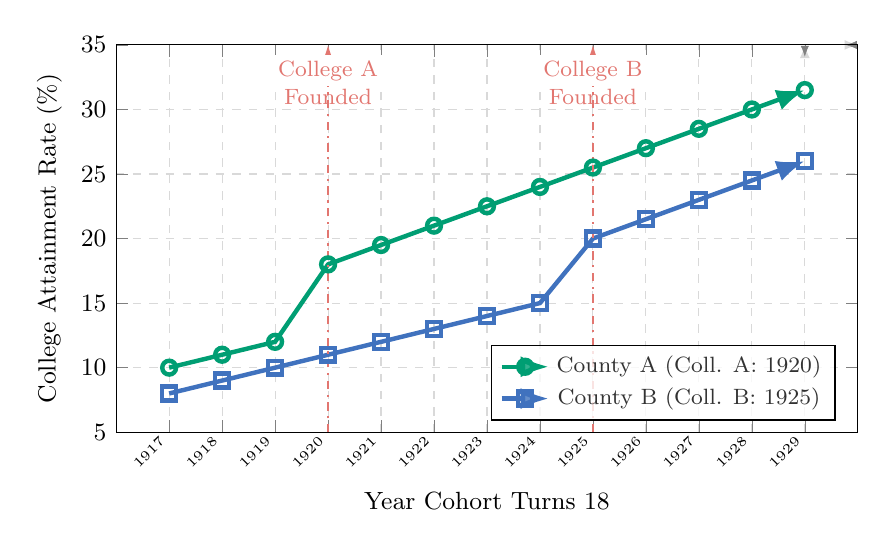
\begin{tikzpicture}

% Define colors
\definecolor{countyA}{RGB}{0,158,115}  % Green color
\definecolor{countyB}{RGB}{64, 114, 190}  % Blue color

\begin{axis}[
    width=11cm,
    height=6.5cm,
    xlabel={Year Cohort Turns 18},
    ylabel={College Attainment Rate (\%)},
    xlabel style={font=\small},
    ylabel style={font=\small},
    xmin=1916,
    xmax=1930,
    ymin=5,
    ymax=35,
    xtick={1917,1918,1919,1920,1921,1922,1923,1924,1925,1926,1927,1928,1929},
    xticklabels={1917,1918,1919,1920,1921,1922,1923,1924,1925,1926,1927,1928,1929},
    x tick label style={rotate=45, anchor=east, font=\tiny},
    ytick={5,10,15,20,25,30,35},
    yticklabel style={font=\small},
    grid=major,
    grid style={dashed, gray!30},
    legend pos=south east,
    legend style={font=\footnotesize, fill=white, fill opacity=0.8, draw=black},
]

% County A - Actual line (University A founded 1920)
\addplot[
    countyA,
    ultra thick,
    mark=o,
    mark size=2.5pt,
    solid
] coordinates {
    (1917, 10)
    (1918, 11)
    (1919, 12)
    (1920, 18)  % Jump at founding
    (1921, 19.5)
    (1922, 21)
    (1923, 22.5)
    (1924, 24)
    (1925, 25.5)
    (1926, 27)
    (1927, 28.5)
    (1928, 30)
    (1929, 31.5)
};
\addlegendentry{County A (Coll. A: 1920)}

% County B - Actual line (University B founded 1925)
\addplot[
    countyB,
    ultra thick,
    mark=square,
    mark size=2.5pt,
    solid
] coordinates {
    (1917, 8)
    (1918, 9)
    (1919, 10)
    (1920, 11)  % No jump - no university yet
    (1921, 12)
    (1922, 13)
    (1923, 14)
    (1924, 15)
    (1925, 20)  % Jump at founding
    (1926, 21.5)
    (1927, 23)
    (1928, 24.5)
    (1929, 26)
};
\addlegendentry{County B (Coll. B: 1925)}

% Vertical lines for university founding years
\draw[thick, red!70, dashdotted] (axis cs:1920,5) -- (axis cs:1920,35);
\draw[thick, red!70, dashdotted] (axis cs:1925,5) -- (axis cs:1925,35);

% Labels for university founding - placed at the top with arrows
\node[red!70, font=\footnotesize, fill=white, inner sep=2pt] at (axis cs:1920,33) {College A};
\node[red!70, font=\footnotesize, fill=white, inner sep=2pt] at (axis cs:1925,33) {College B};
\node[red!70, font=\footnotesize] at (axis cs:1920,31) {Founded};
\node[red!70, font=\footnotesize] at (axis cs:1925,31) {Founded};

% DD estimate annotation
\draw[decoration={brace, amplitude=5pt}, decorate, thick]
    (axis cs:1916,28) -- (axis cs:1916,33);
\node[left, align=left, font=\footnotesize] at (axis cs:1915.5,30.5) 
    {DD = $(\Delta_A^{1920} - \Delta_B^{1920})$\\
     \small Treatment effect\\
     \small of Univ. A};
\end{axis}
\end{tikzpicture}
\end{frame}

\begin{frame}[label=baseline]{Effect of college founding on college attendance}
  \begin{figure}
        \centering
        \includegraphics[width=0.8\textwidth,height=0.7\textheight,keepaspectratio]{"/Users/cjwardius/Library/CloudStorage/OneDrive-UCSanDiego/demo of education/output/figures/twfe_college_attainment_baseline.png"}
        \caption{Standard errors clustered at the county level. All specifications include birth year, county, nativity, race, mother's birth place, father's birth place, and sex fixed effects along with controls for pre-18 residential moves.}
    \end{figure}
\end{frame}



\begin{frame}[label=robustness]{Robustness exercises}
  \begin{wideitemize}
    \item TWFE variation in treatment timing bias \hyperlink{borusyak}{\beamerbutton{here}}
    \item Controlling for county-by-cohort linear time trends \hyperlink{county_trends}{\beamerbutton{here}}
    \item Restricting the sample to only counties that have minimum 30 observations in each age bin \hyperlink{min30}{\beamerbutton{here}}
    \item Placebo test comparing attainment of individuals born before versus far before the college founding \hyperlink{placebo}{\beamerbutton{here}}
  \end{wideitemize}
\end{frame}

\begin{frame}[label=next_steps]{Next steps}
  \begin{enumerate}
    \item \textbf{Heterogeneity analysis}
      \begin{enumerate}
        \item On the person-side, estimate effects by race, sex, and parent's income
        \item On the college-side, estimate effects by junior versus conventional college and state versus non-state college
        \item Complementarity in investment between HS education spending and college founding
      \end{enumerate}
    \item \textbf{Other identification exercises on the effect of college expansion on attainment}
      \begin{enumerate}
        \item Incorporate demographic-specific college expansions \hyperlink{demo_specific}{\beamerbutton{here}}
        \item Incorporate distance from college founding
      \end{enumerate}
  \item \textbf{Data}
  \begin{enumerate}
    \item Fully digitize the Biennial Surveys / Commissioner's Reports on Higher Education
  \end{enumerate}
  \item \textbf{Model}
  \begin{enumerate}
    \item Write down a two-stage model where individuals (1) invest in education then (2) migrate for work. College expansions decrease the cost of education. \hyperlink{model}{\beamerbutton{rough sketch}}
  \end{enumerate}
\end{enumerate}
\end{frame}


\begin{frame}
  \centering
  cwardius@ucsd.edu
  \Huge
  $\reversemathwitch*$
\end{frame}



\appendix
\setbeamertemplate{headline}{}


\begin{frame}[label=regional_trends_k_12_expend]{Regional trends in K-12 spending per capita}
  \begin{figure}
        \centering
        \includegraphics[width=0.8\textwidth,height=0.7\textheight,keepaspectratio]{"/Users/cjwardius/Library/CloudStorage/OneDrive-UCSanDiego/demo of education/output/figures/k12_expenditure_by_region.png"}
    \end{figure}
    \centering
    \hyperlink{west_focuses_on_public}{\beamerbutton{Back to slide}}
\end{frame}


\begin{frame}[label=regional_junior_foundings]{Regional trends in K-12 spending per capita}
  \begin{figure}
        \centering
        \includegraphics[width=0.8\textwidth,height=0.7\textheight,keepaspectratio]{"/Users/cjwardius/Library/CloudStorage/OneDrive-UCSanDiego/demo of education/output/figures/junior_colleges_per_capita_by_region_decade.png"}
    \end{figure}
    \centering
    \hyperlink{west_focuses_on_public}{\beamerbutton{Back to slide}}
\end{frame}


\begin{frame}[label=spatialstability]{County spatial stability over 1900-1940}
    \input{"/Users/cjwardius/Library/CloudStorage/OneDrive-UCSanDiego/demo of education/output/tables/county_boundary_overlap.tex"}

    \vspace{1em}
    \centering
    \hyperlink{isolating}{\beamerbutton{Back to Isolating treated and control counties}}
\end{frame}


\begin{frame}[label=countycrosswalk]{Creating a county crosswalk}
We need consistent county boundaries to accurately assign which people experience a college creation versus which do not.
\vspace{.5cm}

\textbf{Approach:}
\begin{enumerate}
\item Use 1940 as the reference year
\item Spatially intersect 1900, 1910, 1920, and 1930 boundaries with 1940 boundaries
\item Match counties where the intersection exceeds 70\% overlap
\item Retain only counties that appear consistently across all census years
\end{enumerate}
\vspace{1em}
\centering
\hyperlink{isolating}{\beamerbutton{Back to Isolating treated and control counties}}
\end{frame}


\begin{frame}[label=borusyak]{Effects adjusting for treatment effect heterogeneity: \cite{borusyakRevisitingEventStudyDesigns2024}}
  \begin{figure}
        \centering
        \includegraphics[width=0.8\textwidth,height=0.7\textheight,keepaspectratio]{"/Users/cjwardius/Library/CloudStorage/OneDrive-UCSanDiego/demo of education/output/figures/did_imputation_college_attainment_baseline.png"}
    \end{figure}
    \centering
    \hyperlink{robustness}{\beamerbutton{Back to robustness}}
\end{frame}


\begin{frame}[label=county_trends]{Effects controlling for county-by-cohort linear trends}
  \begin{figure}
        \centering
        \includegraphics[width=0.8\textwidth,height=0.7\textheight,keepaspectratio]{"/Users/cjwardius/Library/CloudStorage/OneDrive-UCSanDiego/demo of education/output/figures/twfe_college_attainment_county_trends.png"}
    \end{figure}
    \centering
    \hyperlink{robustness}{\beamerbutton{Back to robustness}}
\end{frame}

\begin{frame}[label=min30]{Effects restricting the sample to counties with more than 30 observations in each age bin}
  \begin{figure}
        \centering
        \includegraphics[width=0.8\textwidth,height=0.7\textheight,keepaspectratio]{"/Users/cjwardius/Library/CloudStorage/OneDrive-UCSanDiego/demo of education/output/figures/twfe_college_attainment_minimum30_in_bin.png"}
    \end{figure}
    \centering
    \hyperlink{robustness}{\beamerbutton{Back to robustness}}
\end{frame}


\begin{frame}[label=placebo]{Placebo test comparing attainment of individuals born before versus far before the college founding}
  \begin{figure}
        \centering
        \includegraphics[width=0.8\textwidth,height=0.7\textheight,keepaspectratio]{"/Users/cjwardius/Library/CloudStorage/OneDrive-UCSanDiego/demo of education/output/figures/placebo_twfe_college_attainment_baseline.png"}
    \end{figure}
    \centering
    \hyperlink{robustness}{\beamerbutton{Back to robustness}}
\end{frame}


\begin{frame}[label=demo_specific]{Demographic-specific college foundings}
  \begin{figure}
 \includegraphics[scale=.4]{"/Users/cjwardius/Library/CloudStorage/OneDrive-UCSanDiego/demo of education/output/figures/demographic_specific_colleges_1900_1940.png"}   
  \end{figure}
  \centering
  \hyperlink{next_steps}{\beamerbutton{Back to next steps}}
\end{frame}
 
\begin{frame}[label=model]{Model-implied estimating equations}
\cite{hsiaoEducationalInvestmentSpatial2024} model implied estimating equation, $j$: origin, $k$ birth cohort, $l$ destination
\begin{align}
  \log \bar w_{jkl} - \log \bar e_{jk} = \log\frac{\tilde \epsilon}{\bar\epsilon} - \log a_l + \log \tau_{jk}^e + \log \tau^m_{jkl}
\end{align}
From which $\tau_{jk}^e$, the cost of education, can be estimated. Use the Cohort DD from earlier as a source of quasi-experimental variation in education costs:
\begin{align}
  \log \tau_{jk}^e = \alpha_j + \alpha_k + \beta S_j T_k +\epsilon_{jk}
\end{align}
where $S_j = 1$ if $j$ received a new college and $S_k=1$ if $k$ was ``exposed'' to the college founding.

\centering
\hyperlink{next_steps}{\beamerbutton{back to next steps}}
\end{frame}




\end{document}

